%
%

\multiproblem{triangle}{
  Consider the triangular load distribution shown here:
  \begin{center}
    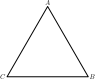
\includegraphics{triangle.pdf}
  \end{center}
  \begin{enumerate}
    \item Find an equation for the distributed force $w(x)$.
    \item Find the total force and moment around $A$ of $w(x)$ and hence find
      the reactions $R_A$ and $M_A$.
    \item If there were a point force equivalent to $w(x)$ (for external force
      and moment balance) what would it be and where would it act?
    \item Find the shear stress $V(x)$ and bending moment $M(x)$ throughout
      the beam. Verify that your solutions satisfy the correct boundary
      conditions at both ends of the beam.
  \end{enumerate}
}

\multiproblem{rectangle}{
  Repeat the above calculations for the rectangular load distribution shown
  here:
  \begin{center}
    \includegraphics{rectangle.pdf}
  \end{center}
}

\multiproblem{point}{
  Find the bending moment and shear stress throught the beam shown here:
  \begin{center}
    \includegraphics{point_distributed.pdf}
  \end{center}
}

\multiproblem{diving}{
  Consider this arrangement:
  \begin{center}
    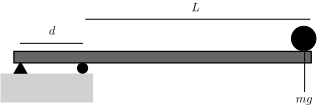
\includegraphics{diving.pdf}
  \end{center}
  \begin{enumerate}
    \item Find the reaction forces at the two supports resulting from the
      large weight at the end of the beam (assume the beam has zero mass).
    \item Find shear stress and bending moment throughout the length of the
      beam.
    \item Repeat the calculations taking account of the weight of the beam.
      Assume it has mass $m_b \neq 0$.
  \end{enumerate}
}

\multiproblem{bridge}{
  Repeat the above calculations for this bridge (both for zero and non-zero
  beam mass):
  \begin{center}
    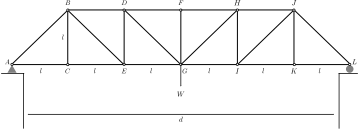
\includegraphics{bridge.pdf}
  \end{center}
}
